\usecaseristoratore{Visualizzazione stato di pagamento}
\label{usecase:Visualizzazione stato di pagamento}

\begin{figure}[h]
	\centering
	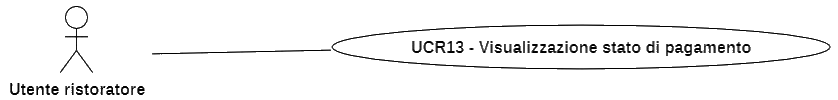
\includegraphics[width=0.9\textwidth]{./uml/UCR13.png} 
	\caption{Visualizzazione stato di pagamento}
	\label{fig:UCR13}
  \end{figure}

\begin{itemize}
	
    \item \textbf{Attore principale:} Utente ristoratore.

	\item \textbf{Precondizione:} L'Utente ristoratore sta visualizzando la lista delle ordinazioni di una prenotazione (vedi \autoref{usecase:Visualizzazione lista ordinazioni}).

	\item \textbf{Postcondizione:} L'Utente ristoratore visualizza lo stato del pagamento di un ordinazione.

	\item \textbf{Scenario principale:}
	\begin{enumerate}
		\item Il Sistema mostra per ogni ordinazione presente all'interno della prenotazione lo stato di pagamento, che può essere:
        \begin{itemize}
            \item Da pagare.
            \item Pagato.
        \end{itemize}
        \item L'Utente ristoratore visualizza per ogni ordinazione lo stato del pagamento.
	\end{enumerate}

\end{itemize}